%% LyX 1.1 created this file.  For more info, see http://www.lyx.org/.
%% Do not edit unless you really know what you are doing.
\documentclass[12pt,english]{article}
\usepackage[T1]{fontenc}
\usepackage[latin1]{inputenc}
\usepackage{babel}
\usepackage{graphics}
\usepackage{verbatim}

\makeatletter

%%%%%%%%%%%%%%%%%%%%%%%%%%%%%% LyX specific LaTeX commands.
\providecommand{\LyX}{L\kern-.1667em\lower.25em\hbox{Y}\kern-.125emX\@}

%%%%%%%%%%%%%%%%%%%%%%%%%%%%%% Textclass specific LaTeX commands.
 \newcommand{\lyxaddress}[1]{
   \par {\raggedright #1 
   \vspace{1.4em}
   \noindent\par}
 }

\makeatother
\begin{document}

\title{SAM: A computer code for nuclear scattering at intermediate and high
energies}


\author{R. Crespo and A.M. Moro}

\maketitle

\lyxaddress{Departamento de F\textbackslash{}'\{\textbackslash{}i\}sica, Instituto
Superior T\textbackslash{}'ecnico, 1049-001 Lisboa, Portugal}


\lyxaddress{Email:raquel@wotan.ist.utl.pt, moro@mary.ist.utl.pt}


\subsection*{PROGRAM SUMMARY}

\begin{verse}
\emph{Title of the program}: \textbf{SAM} (\textbf{S}cattering \textbf{AM}plitudes)

\emph{Program obtained from:} CPC Program Library, Queen's University
of Belsfast, N. Ireland

\emph{Computers:} The code runs in UNIX machines

\emph{Operating systems:} UNIX

\emph{Program language used:} Fortran-90

\emph{Memory required to execute with typical data}:

\emph{Keywords:} NN, nucleon-nucleus, nucleus-nucleus, Many-body,
Few-body, Multiple scattering, elastic, inelastic, breakup.

\emph{Nature of physical problem:}
\end{verse}

\subsection*{LONG WRITE-UP}

\tableofcontents{}


\section{Introduction}

The basic idea of this code is to assemble few-body and many-body
aspects of the scattering from an \emph{abinitio} point of view. The
fundamental dynamical and struture inputs are the nucleon-nucleon
(NN) transition amplitude, and the nucleus wave function respectively. 

It gathers and extends previous existing main fortran-77 codes and
exploits the new capabilities of fortran90. It consistes of 3 main
blocks: NNamp, MSOamp and MSTamp. Some utility codes were also included
such as Dfold, Espectrum and Fit. 

NNamp evaluates the on- and off- energy shell free nucleon-nucleon
(NN) scattering amplitudes in the momentum space configuration from
a realistic NN interaction such as Paris or Bonn \cite{Lacombe80,Machleidt87}.
It extends the work of \cite{Redish87a,Redish87b,Redish87c} to include
all components of the NN scattering amplitude in the Wolfenstein parametrization
\cite{Wolfenstein52,Crespo91  } and in the tensor representation
\cite{Crespo02a}.

MSOamp evaluates the elastic scattering observables for nucleon-nucleus
elastic scatering from an optical potential in the momentum space
configuration. The optical potential is constructed as a multiple
scattering expansion in terms of the free NN transition amplitude
to second order evaluated at the appropriate energy as formulated
in \cite{Ker59,Wat53,Crespo92} and implemented numerically in \cite{Landau82,Crespo91  }.
Within the single scattering approximation the optical potential essentially
probes the target nucleus density. Higher order terms depend on the
target correlation function.

The free off- the energy shell NN transition amplitude, used in MSOamp
is obtained form NNamp. The target densities are evaluated either
from an Harmonic Oscillator model, parameter-Fermi distribution or
read externally.

MSTamp evaluates the multiple scattering expansion of total transition
amplitude for nucleon scattering from a system well described by two
and three loosely bound sub-systems in terms of each projectile-subsystem
scattering amplitude. The scattering from a cluster of nucleons is
calculated with MSOamp, or read externally, and the scattering from
a valence nucleon subsystem is calculated with NNamp.


\section{Scattering framework}

We consider the scattering of a projectile from a target consisting
of \( \mathcal{N} \) sub-systems. The subsystems \( \mathcal{I},\mathcal{J} \)
... are assumed to be stable and can be either composite nuclei or
nucleons. The total transition amplitude for the scattering is

\begin{equation}
\label{Tmat}
T=V+VGT
\end{equation}
 with \( V=\sum v_{_{}\mathcal{I}} \)is the interaction between the
projectile and each subsystem. In this equation, \( G=(E^{+}-K_{0}-H_{0})^{-1} \)is
the propagator with \( K_{0} \) the kinetic energy for the projectile
in the center of mass of the interacting P-T system, and \( H_{0} \)
the target nucleus Hamiltonian. This is a many-body problem, and two
distinct multiple scattering approaches can be followed:


\subsubsection*{The Multiple Scattering expansion of the total Transition amplitude
(MST):}

In this approach, the total transition amplitude eq.(\ref{Tmat})
is rewritten as

\begin{equation}
\label{Tmat-i}
T=\sum ^{\mathcal{N}}_{\mathcal{I}=1}T_{\mathcal{I}},
\end{equation}
where \( T_{\mathcal{I}} \) satisfies

\begin{equation}
T_{\mathcal{I}}=\tau _{\mathcal{I}}+\tau _{\mathcal{I}}G\sum _{\mathcal{J}\neq \mathcal{I}}T_{\mathcal{J}},
\end{equation}
In here, \( \tau _{\mathcal{I}} \) is the projectil-subsystem \( \mathcal{I} \)
transition amplitude

\begin{equation}
\tau _{\mathcal{I}}=v_{\mathcal{I}}+v_{\mathcal{I}}G\tau _{\mathcal{I}}.
\end{equation}
In this scattering framework, elastic and inelastic channels are treated
in equal footing. However, rapid convergence is only expected for
the case of loosely bound systems for projectile scattering in the
intermediate energy region.


\subsubsection*{The Multiple Scattering expansion of the Optical potential (MSO):}

Equivalently, we can rewrite eq. (\ref{Tmat-i}) in terms of an optical
potential by projecting the intermediate states of (\ref{Tmat-i})
into the ground state. If couplings to inelastic channels are small,
we expect that higher order terms of the optical potential give a
negligeable contribution to the scattering. The key problem in here
is how to handle antisymmetrization. The multiple scattering formalism
develloped by Kermann, McMannus and Thaler \cite{Ker59}, is adequate
for studying the scattering of a nucleon projectile fom a system of
A nucleons. It works in the antisymmetrized space of target nucleus
and neglets three body target exchange processes between a projectile
nucleon and two particles at the target. This contribution is expected
to be small for projectile energies in the intermediate energy region.
In this formalism the scattering observables are calculated in terms
of the transition amplitude

\begin{equation}
T=\frac{A}{A-1}T(U^{KMT})
\end{equation}
Here, \( T(U^{KMT}) \) is the transition operator generator by the
optical potential \( U^{KMT} \),

\begin{equation}
\label{T-KMT}
T=U^{KMT}+U^{KMT}GT
\end{equation}
 The optical potential \( U^{KMT} \)can be written as an expansion
in terms of the NN transition amplitude 

\begin{equation}
\label{Uopt-KMT}
U^{KMT}=U^{(0)}[1+\mathcal{A}GQ_{0}U]=U^{(0)}[1+\mathcal{A}GQ_{0}U^{(0)}+\cdots ]
\end{equation}
where \( \mathcal{A} \)is the antisymetrization operator for the
A target nucleons. The Pauli blocking operator \( Q_{0} \) projects
off the target ground state \( \phi _{0} \), i.e. \( Q_{0}=1-P_{0} \)
where \( P_{0}=|\phi _{0}\rangle \langle \phi _{0}| \). In eq.(\ref{Uopt-KMT})
\( U^{(0)}=(A-1)\tau _{01}(E) \), where \( \tau _{01} \)is the antisymmetrized
effective NN transition operator, which describes the scattering of
the projectile with any one of the target nucleons (labelled '1'),

\begin{equation}
\tau _{01}(E)=v_{01}+v_{01}\mathcal{A}G\tau _{01}(E)
\end{equation}
The presence of the antisymmetrization operator allows only physical
states of the nucleus as intermediate states. If one introduces the
NN transition operator 

\begin{equation}
\hat{t}_{01}(E)=v_{01}+v_{01}G\hat{t}_{01}(E)
\end{equation}
which is not that describing the free NN scattering since the propagator
remains a many-body operator, then the optical potential for elastic
scattering, to second order in \( \hat{t}_{01} \)is given as

\begin{equation}
\label{Uopt-SSA+DSA}
U^{opt}=\langle \phi _{0}|U^{KMT}|\phi _{0}\rangle =U_{SSA}^{opt}+U_{DSA}^{opt}
\end{equation}
with the single scattering term given as

\begin{equation}
\label{Uopt-SSA}
U_{SSA}^{opt}=(A-1)\langle \phi _{0}|\hat{t}_{01}(E)|\phi _{0}\rangle ,
\end{equation}
and the double scattering

\begin{equation}
\label{Uopt-DSA}
U_{DSA}^{opt}=-(A-1)^{2}\langle \phi _{0}|\hat{t}_{01}(E)P_{0}G_{0}\hat{t}_{01}(E)|\phi _{0}\rangle +\frac{A-1}{A}\sum _{i\neq j}\langle \phi _{0}|\hat{t}_{0i}(E)G\hat{t}_{0j}(E)|\phi _{0}\rangle .
\end{equation}
with the Green's function \( G_{0}=(E-K_{0}+i\epsilon )^{-1} \).


\section{Adopted conventions}

Multiple scattering frameworks are conveniently handled in the momentum
space configuration. Through this work we adopt plane wave states
\( |\vec{k}\rangle  \) normalized such that

\begin{equation}
\langle \vec{r}|\vec{k}\rangle =\frac{1}{(2\pi )^{3/2}}\exp (i\vec{k}\cdot \vec{r}).
\end{equation}
The plane wave states can be expanded in terms of the angular momentum
basis states \( |k(LS)JM\rangle  \) 

\begin{equation}
\label{partialk}
|\vec{k}\rangle =\sqrt{\frac{2}{\pi }}\sum _{JLSM}i^{L}|k(LS)JM\rangle Y_{JL}^{M+}(\hat{k}),
\end{equation}
where \( Y_{JL}^{M+}(\hat{k}) \) is the spin sherical harmonics for
spin S, and where the angular momentum basis satisfies the orthogonal
relation 

\begin{equation}
\langle k'(LS)JM|k(LS)JM\rangle =\frac{\pi }{2}\frac{\delta (k-k')}{k^{2}}.
\end{equation}



\section{NN amplitudes}

We consider the scattering of an incident (0) and struck (1) nucleons.
Within a non-relativistic potential picture, thet interact via a two-body
potential, \( v_{01} \). The nucleon-nucleon (NN) transition operator
satisfies the integral equation

\begin{equation}
t_{01}(E)=v_{01}+v_{01}\frac{1}{E-\hat{K}_{0}-\hat{K}_{1}-i\epsilon }t_{01}(E),
\end{equation}
with \( \hat{K}_{0} \) and \( \hat{K}_{1} \) the momentum operator
of particles '0' and '1' respectively. The free NN scattering amplitude
\( M(\omega ,\vec{\mathcal{K}}',\vec{\mathcal{K}}) \), describing
the scattering from two-nucleon states with relative momenta \( \vec{\mathcal{K}} \)
and \( \vec{\mathcal{K}}' \) for relative energy \( \omega  \) in
their centre of mass (cm) frame, is related to the anti-symmetrised
transition matrix elements by \begin{eqnarray}
M(\omega ,\vec{\mathcal{K}}',\vec{\mathcal{K}})=\langle \vec{\mathcal{K}}'|M(\omega )|\vec{\mathcal{K}}\rangle =-\frac{4\pi ^{2}\mu }{\hbar ^{2}}\langle \vec{\mathcal{K}}'|t^{f}_{01}(\omega )|\vec{\mathcal{K}}\rangle , & \label{scattA} 
\end{eqnarray}
 where \( \mu  \) the NN reduced mass. For ease of notation, we shall
drop whenever convenient the explicit dependence on the relative energy
\( \omega  \). The scattering amplitude is an operator in both the
NN spin and isospin spaces. There exist a few ways to explicitize
this dependence. The Wolfenstein representation \cite{Wolfenstein52}
the amplitude is expressed in terms of six components, the coefficients
of spin operators which are scalar products of the Pauli spin vectors
\textbackslash{}vec\{\textbackslash{}sigma \}\_\{i\} for the projectile
and struck nucleons with a set of unit vectors defined by the scattering
plane of the nucleon pair. Equivalently, it can be expressed in terms
of central, spin-orbit and usual tensor components \cite{Love81,Love85}.
Alternatively it can be represented in terms of irreducible tensor
operators in the space of spin S(=0,1) of the interacting pair as
in \cite{Hooton71} and \cite{Crespo02a}.We shall discuss some of
these representations in detail later on. In any case, the coefficients
of the spin operators are evaluated from the decomposition of the
NN amplitude of Eq.\ (\ref{scattA}) into spin singlet (\( S=0 \))
and triplet (\( S=1 \)) components, \( M^{S}_{\nu' \nu } \), where
\( \nu  \) and \( \nu'  \) refer to the incident and final state
spin projections in state \( S \)\begin{eqnarray}
\langle \vec{\mathcal{K}}'|M|\vec{\mathcal{K}}\rangle =\sum _{S\nu \nu' }M^{S}_{\nu' \nu }(\vec{\mathcal{K}}',\vec{\mathcal{K}})|S\nu' \rangle \langle S\nu |.
\end{eqnarray}
 These \( M^{S}_{\nu' \nu }=\langle \vec{\mathcal{K}}'S\nu' |M|\vec{\mathcal{K}}S\nu \rangle  \)
are in turn calculated during the construction of the NN amplitudes
from the partial wave transition amplitudes \( M^{JS}_{L'L}({\mathcal{K}}',{\mathcal{K}}) \).
We adopt the convention that \begin{eqnarray}
\langle \vec{\mathcal{K}}'|M|\vec{\mathcal{K}}\rangle  & = & \frac{2}{\pi }\sum _{JLL'SM}i^{L-L'}{\mathcal{Y}}^{M}_{(L'S)J}(\hat{\mathcal{K}}')M^{JS}_{L'L}({\mathcal{K}}',{\mathcal{K}})\nonumber \\
 & \times  & {\mathcal{Y}}^{M\dagger }_{(LS)J}(\hat{\mathcal{K}}),
\end{eqnarray}
 where \( {\mathcal{Y}}^{M}_{(LS)J} \) is a spin-angle function \begin{eqnarray}
{\mathcal{Y}}^{M}_{(LS)J}(\hat{\mathcal{K}}')=\sum _{\Lambda \nu }(L\Lambda S\nu |JM)Y_{L\Lambda }(\hat{\mathcal{K}}'){\mathcal{X}}_{S\nu },
\end{eqnarray}
 and \( Y_{L\Lambda } \) and \( {\mathcal{X}}_{S\nu } \) are spherical
harmonics \cite{Brink} and total spinors of the NN pair. Explicitly
therefore \begin{eqnarray}
M^{S}_{\nu' \nu }(\vec{\mathcal{K}}',\vec{\mathcal{K}}) & = & \frac{2}{\pi }\sum _{JMLL'\Lambda \Lambda' }i^{L-L'}(L'\Lambda' S\nu' |JM)\nonumber \\
 & \times  & (L\Lambda S\nu |JM)Y_{L'\Lambda' }(\hat{\mathcal{K}}')Y^{*}_{L\Lambda }(\hat{\mathcal{K}})\nonumber \\
 & \times  & M^{JS}_{L'L}({\mathcal{K}}',{\mathcal{K}}).\label{msnn} 
\end{eqnarray}
 The partial wave sums are, of course, over values which satisfy the
Pauli principle requirement, \( L+S+T \)=odd. Explicit expressions
can be found in Appendix C of \cite{Crespo92} 


\subsection{The Wolfenstein representation}

The Wolfenstein decomposition of the NN amplitude for the scattering
of an incident (0) and struck (1) nucleon \cite{Wolfenstein52}, has
been used extensively. It writes the most general form of the amplitude,
consistent with time-reversal, parity, and rotational invariance,
as \begin{eqnarray}
M(\omega ,\vec{\mathcal{K}}',\vec{\mathcal{K}}) & = & {\mathcal{A}}+{\mathcal{B}}(\vec{\sigma }_{0}\cdot \hat{n})(\vec{\sigma }_{1}\cdot \hat{n})+{\mathcal{C}}(\vec{\sigma }_{0}+\vec{\sigma }_{1})\cdot \hat{n}\nonumber \\
 & + & {\mathcal{D}}(\vec{\sigma }_{0}\cdot \hat{m})(\vec{\sigma }_{1}\cdot \hat{m})+{\mathcal{E}}(\vec{\sigma }_{0}\cdot \hat{\ell }\, )(\vec{\sigma }_{1}\cdot \hat{\ell }\, )\nonumber \\
 & + & {\mathcal{F}}[(\vec{\sigma }_{0}\cdot \hat{\ell }\, )(\vec{\sigma }_{1}\cdot \hat{m})+(\vec{\sigma }_{1}\cdot \hat{m})(\vec{\sigma }_{0}\cdot \hat{\ell }\, )]\label{KMT} 
\end{eqnarray}
 where the orthogonal set of unit vectors \( \hat{n}=(\vec{\mathcal{K}}\times \vec{\mathcal{K}}')/|\vec{\mathcal{K}}\times \vec{\mathcal{K}}'| \),
\( \hat{\ell }=(\vec{\mathcal{K}}'+\vec{\mathcal{K}})/|\vec{\mathcal{K}}'+\vec{\mathcal{K}}| \),
and \( \hat{m}=\hat{\ell }\times \hat{n} \) are defined by the NN
scattering plane \cite{Wolfenstein52}. The coefficient amplitudes
\( {\mathcal{A}},\ldots {\mathcal{F}} \) can also be expressed as
complex functions of the energy \( \omega =\hbar ^{2}k^{2}_{0}/2\mu  \),
the momentum transfer \( \vec{q}=(\vec{\mathcal{K}}'-\vec{\mathcal{K}}) \)
and the total momentum \( \vec{\mathcal{Q}}=(\vec{\mathcal{K}}+\vec{\mathcal{K}}')/2 \)
of the NN pair in their cm frame. 

They remain operators in isotopic spin space, so for instance \begin{eqnarray}
{\mathcal{A}}(\omega ,\vec{q},\vec{\mathcal{Q}}) & = & {\mathcal{A}}_{0}+{\mathcal{A}}_{\tau }(\vec{\tau }_{0}\cdot \vec{\tau }_{1})\nonumber \\
 & = & {\mathcal{A}}^{T=0}P_{0}+{\mathcal{A}}^{T=1}P_{1},\label{tautau} 
\end{eqnarray}
 To express the coefficient amplitudes \( {\mathcal{A}},\ldots {\mathcal{F}} \)
in terms of spin amplitudes \( M^{S}_{\nu \nu '} \)it is necessary
to make a choice for the axis of quantization axis. Taking this axis
along the incident beam direction (\( \vec{\mathcal{K}}) \) then

\begin{equation}
4{\mathcal{A}}=(2M^{1}_{11}+M^{1}_{00}+M^{0}_{00})
\end{equation}
 \begin{equation}
4{\mathcal{B}}=(M^{1}_{00}-M^{1}_{1-1}-M^{0}_{00})
\end{equation}


\begin{equation}
4{\mathcal{C}}=i(M^{1}_{10}-M^{1}_{01})/2\sqrt{2}
\end{equation}
and

\begin{equation}
4{\mathcal{D}}=2(y+2x-1)M^{1}_{11}-\sqrt{8xy}(M^{1}_{10}+M^{1}_{01})+2yM^{1}_{1-1}+(2y-1)M^{1}_{00}-M^{0}_{00}
\end{equation}


\begin{equation}
{\mathcal{E}}=2(x+2y-1)M^{1}_{11}-\sqrt{8xy}(M^{1}_{10}+M^{1}_{01})+2xM^{1}_{1-1}+(2x-1)M^{1}_{00}-M^{0}_{00}
\end{equation}


\begin{equation}
{\mathcal{F}}=\sqrt{xy}(M^{1}_{11}-M^{0}_{00}-M^{1}_{1-1})+\sqrt{2}(x-y)(M^{1}_{10}+M^{1}_{01})
\end{equation}
where \( \theta =cos^{-1}({K}\cdot {K}'/|{K}\cdot {K}'|) \) is the
NN center-of-mass scattering angle. In these equations, \( x={N}{K}'^{2}sin^{2}\theta  \)
and \( y={N}({K}+{K}')^{2} \)with \( {N}=1/|{K}+{K}'|^{2} \).


\subsection{The tensor representation}

The tensor representation \cite{Crespo02a} is a a convenient general
method to express the NN transition amplitude as a linear combination
for the spherical components of the spin operators of the two interacting
particles. This is a more treatable representation to be used in multiple
scattering formalisms which required a full treatment of the spin
of the NN transition amplitude. In this representation, the scattering
amplitude is written in terms of the tensor of rank \( \kappa  \)

\begin{eqnarray}
{\mathcal{T}}_{\kappa q}(a,b)=\sum _{\alpha \beta }(a\alpha b\beta |\kappa q)\tau _{a\alpha }(s_{0})\tau _{b\beta }(s_{1}).\label{bigT} 
\end{eqnarray}
 as, \begin{eqnarray}
\langle \vec{\mathcal{K}}'|M|\vec{\mathcal{K}}\rangle =\sum _{\kappa qab}M^{(ab)}_{\kappa q}(\vec{\mathcal{K}}',\vec{\mathcal{K}}){\mathcal{T}}^{\dagger }_{\kappa q}(a,b), & 
\end{eqnarray}
 where \( \tau _{a\alpha }(s_{0}) \) is the irreducible tensor operator
for the projectile particle (0) with spin \( s_{0} \) (\( a=0,\ldots 2s_{0} \));
\( \tau _{b\beta }(s_{1}) \) is the irreducible tensor operator for
the struck particle (1) with spin \( s_{1} \) (\( b=0,\ldots 2s_{1} \)).
Explicitly, since \( \scriptstyle s_{0}=s_{1}={\frac{1}{2}} \), \begin{eqnarray}
\scriptstyle \tau _{00}({\frac{1}{2}})=1,\tau _{1\beta }({\frac{1}{2}})=\sigma _{\beta }(1),
\end{eqnarray}
 with \( \sigma _{\beta }(1) \) the spherical components of \( \vec{\sigma }_{1} \)
with respect to the chosen \( z \)-axis. The scattering amplitudes
\( M^{(ab)}_{\kappa q}(\vec{\mathcal{K}}',\vec{\mathcal{K}}) \) are
calculated from the spin components \( M^{S}_{\nu' \nu }(\vec{\mathcal{K}}',\vec{\mathcal{K}}) \)
according to \cite{Crespo02a}:

\begin{eqnarray}
M^{(ab)}_{\kappa q}(\vec{\mathcal{K}}',\vec{\mathcal{K}})=\sum _{S}M^{S}_{\kappa q}(\vec{\mathcal{K}}',\vec{\mathcal{K}}){\mathcal{N}}^{S}_{\kappa }(ab)
\end{eqnarray}
 with

\begin{eqnarray}
M^{S}_{\kappa q}(\vec{\mathcal{K}}',\vec{\mathcal{K}})=\frac{\hat{\kappa }}{\hat{S}^{2}}\sum _{\nu \nu' }M^{S}_{\nu' \nu }(\vec{\mathcal{K}}',\vec{\mathcal{K}})(S\nu' \kappa q|S\nu ).
\end{eqnarray}
and

\begin{equation}
{\mathcal{N}}^{S}_{\kappa }(ab)=\frac{\hat{S}^{3}\hat{a}\hat{b}}{\hat{s}_{0}\hat{s}_{1}}\left\{ \begin{array}{ccc}
s_{0} & s_{1} & S\\
s_{0} & s_{1} & S\\
a & b & \kappa 
\end{array}\right\} .
\end{equation}
 


\subsection{Partial wave decomposition: solution method}

The spin amplitudes \( M^{S}_{\nu' \nu }=\langle \vec{\mathcal{K}}'S\nu' |M|\vec{\mathcal{K}}S\nu \rangle  \)
used in any of the representations are in directly calculated from
the partial wave transition amplitudes \( M^{JS}_{L'L}({\mathcal{K}}',{\mathcal{K}}) \).
These are evaluated following the procedure detailed in \cite{Red87a}:
In order to deal with the principal value, \( G_{0}^{P} \), in the
intermediate states propagation of the Lippman-Schwinger equation,
the R-matrix is introduced

\begin{equation}
R_{L'L}^{JST}({\mathcal{K}}',{\mathcal{K}})=V^{JST}_{L'L}({\mathcal{K}}',{\mathcal{K}})+\frac{2}{\pi }\sum _{L''}\int ^{\infty }_{0}d{\mathcal{K}}''{\mathcal{K}}''^{2}V_{L'L''}^{JST}({\mathcal{K}}',{\mathcal{K}}'')G_{0}^{P}({\mathcal{K}}'')R_{L''L}^{JST}({\mathcal{K}}'',{\mathcal{K}})
\end{equation}
where \( V^{JST}_{L'L}({\mathcal{K}}',{\mathcal{K}}) \) is the matrix
elements of the NN potential. The principal value is evaluated using
the Sloan method \cite{Sloan68} which consists of using a symmetric
quadrature in the neighbourhood of the pole. The infinite upper limit
of the integral is handled by using a cutoff momentum, which is outside
the region where the dominant contributions occur, and a Gauss-Laguerre
rule for the integration region beyond that cutoff. The partial decomposition
of the transition amplitude can then be related to the R matrix elements
by the Heitler equation:

\begin{equation}
t_{L'L}^{JST}({\mathcal{K}}',{\mathcal{K}})=R_{L'L}^{JST}({\mathcal{K}}',{\mathcal{K}})-2i\mu {\mathcal{K}}_{0}\sum _{l''l'''}R_{L'L''}^{JST}({\mathcal{K}}',{\mathcal{K}}_{0})[1+2i\mu {\mathcal{K}}''R^{JST}({\mathcal{K}}_{0},{\mathcal{K}}_{0})]_{L''L'''}^{-1}R_{l'''l}^{jst}({\mathcal{K}}_{0},{\mathcal{K}})
\end{equation}
 where \( {\mathcal{K}}_{0}=\sqrt{2\mu \omega /\hbar ^{2}} \) is
the NN on- shell momentum.


\section{The MSO amplitudes}


\subsection{The matrix elements of the optical potential }

The Multiple Scattering expansion of the Optical potential formulated
by KMT eq.(\ref{Uopt-SSA+DSA}), can be rewritten as an expantion
in terms of the free NN transition amplitude, \( t_{0i}^{f} \), for
projectile '0' -struck nucleon 'i' scattering \cite{Ker59,Crespo92}.
We assume that the target nucleus of number of mass A is well described
by N clusters, and neglect its total spin.


\subsubsection{The single scattering approximation}

Then, the matrix elements of the SSA to the optical potential in the
momentum space configuration are, using the optimal factorization
or \( t\rho  \) approximation, \begin{equation}
\label{Uopt-SSA-k}
\langle \vec{k}'|U_{SSA}^{opt}|\vec{k}\rangle =\frac{A-1}{A}\sum [\rho ^{i}_{p}(q)\bar{t}_{0p}(\omega ,q,Q/2,\phi )+\rho ^{i}_{n}\bar{t}_{0n}(\omega ,q,Q/2,\phi )]
\end{equation}
where \( \rho ^{i}_{n} \)and \( \rho ^{i}_{p} \)are the nuclear
matter density distributions for the protons and neutrons respectively
for each cluster. Here, \( \bar{t}_{0p} \) and \( \bar{t}_{0n} \)
are the spin averaged proton-proton and neutron-neutron respectively
amplitudes evaluated at the appropriate energy \( \omega =E/2 \),
\( \phi  \) is the angle between the vectors \( \vec{Q}=(\vec{k}'+\vec{k})/2 \)
and \( \vec{q}=(\vec{k}'-\vec{k}) \). Eq. (\ref{Uopt-SSA-k}) can
be rewritten in terms of the central and spin-orbit \emph{off-shell}
Wolfenstein amplitudes. For a spinless target we can write in general

\begin{equation}
\langle \vec{k}'|U_{SSA}^{opt}|\vec{k}\rangle =\langle \vec{k}'|U_{SSA}^{c}|\vec{k}\rangle +i\vec{\sigma }_{0}\cdot \vec{n}\langle \vec{k}'|U_{SSA}^{ls}|\vec{k}\rangle 
\end{equation}
with \( \sigma _{0} \) the spin operator for the projectile and \( \vec{n}=\vec{\kappa }\times \vec{\kappa }'/kk' \),
where

\begin{equation}
\langle \vec{k}'|U_{SSA}^{c}|\vec{k}\rangle =\frac{A-1}{A}\frac{\hbar ^{2}}{4\pi ^{2}\mu }\sum [\rho ^{i}_{p}(q)\mathcal{A}_{0p}(\omega ,q,Q/2,\phi )+\rho ^{i}_{n}\mathcal{A}_{0n}(\omega ,q,Q/2,\phi )],
\end{equation}
and 

\begin{equation}
\langle \vec{k}'|U_{DSA}^{ls}|\vec{k}\rangle =\frac{A-1}{A}\frac{\hbar ^{2}}{4\pi ^{2}\mu }\frac{-i}{sin\theta _{NA}}\sum [\rho ^{i}_{p}(q)\mathcal{C}_{0p}(\omega ,q,Q/2,\phi )+\rho ^{i}_{n}\mathcal{C}_{0n}(\omega ,q,Q/2,\phi )].
\end{equation}
In here, \( \theta _{NA} \)the scattering angle in the nucleon-nucleus
centre of mass frame. Evaluation of the off-shell central and spin-orbit
amplitudes \( \mathcal{A},\mathcal{C}/sin\phi  \), have shown that
for NN relative momenta less than \( 3fm^{-1} \)and \( 50Mev\leq \omega \leq 200Mev \),
they are essentially independent of the variables \( \omega  \) and
\( \phi  \). It is then a good approximation to take this angle to
its on shell value \( \phi =\pi /2 \). At this stage the optical
potential is still non-local. If we further take the total momemtum
to its \emph{on-shell value}, that is

\begin{equation}
Q^{2}=4\mathcal{K}_{0}^{2}-q^{2}\sim [\frac{A+1}{A}k_{0}]^{2}-q^{2}
\end{equation}
then we obtain a local optical potential.

The full folding optical potential for the elastic scattering of protons
from \( ^{16} \)O and \( ^{40} \)O was calculated in the intermediate
energy region \cite{Crespo90a  }, which take into account the folding
of the target density with the NN transition amplitude over the momentum
\( \vec{P}=\frac{\vec{k}+\vec{k}'}{2}-(\mathcal{K}+\mathcal{K}') \)
where \( \vec{k}(\vec{k}') \) is the income (outgoing) momentum of
the projectile in the c.m frame, and \( \mathcal{K}(\mathcal{K}') \)
the relative momenta of the two interacting nucleons. The calculated
observables show that the optimal factorization provides a good approximation
to the optimal factorization in this case \cite{Crespo90a  }.


\subsubsection{The double scattering approximation}

If one uses closure approximation in the intermediate states propagator
of the double scattering term eq. (\ref{Uopt-DSA}) then the second
order contribution can be written in terms of the target correlation
function 

\begin{equation}
D(\vec{r},\vec{r}')=\rho (\vec{r})\rho (\vec{r}')-\rho (\vec{r},\vec{r}')
\end{equation}
where \( \rho (\vec{r}) \) is the target nucleus matter density distribution
normalized to the number of nucleons and \( \rho (\vec{r},\vec{r}') \)
the probability density of finding a nucleon at position \( \vec{r} \),
and another at position \( \vec{r}' \), i.e., 

\begin{equation}
\rho (\vec{r},\vec{r}')=\langle \phi _{0}|\sum _{i\neq j}\delta (\vec{r}-\vec{r}_{i})\delta (\vec{r}'-\vec{r}_{j})|\phi _{0}\rangle 
\end{equation}
 The central component of the double scattering contribution can be
written as:

\begin{equation}
\langle \vec{k}'|U_{DSA}^{c}|\vec{k}\rangle =\langle \vec{k}'|U_{DSA}^{c;I}|\vec{k}\rangle +\langle \vec{k}'|U_{DSA}^{c;II}|\vec{k}\rangle 
\end{equation}
where

\begin{equation}
\langle \vec{k}'|U_{DSA}^{c;I}|\vec{k}\rangle =-\frac{A}{A-1}\int d\vec{k}''\beta (\omega ,\vec{k}',\vec{k}'',\vec{k})g(k'')\int d\vec{r}\int d\vec{r}'\exp -i(\vec{q}\cdot \vec{r}+\vec{q}'\cdot \vec{r}')D(\vec{r},\vec{r}')
\end{equation}
and

\begin{equation}
\langle \vec{k}'|U_{DSA}^{c;II}|\vec{k}\rangle =-(A-1)\int d\vec{k}''\gamma (\omega ,\vec{k}',\vec{k}'',\vec{k})g(k'')\rho (q)\rho (q').
\end{equation}
In these equations

\begin{equation}
\beta (\omega ,\vec{k}',\vec{k}'',\vec{k})=
\end{equation}
and 

\begin{equation}
\gamma (\omega ,\vec{k}',\vec{k}'',\vec{k})=
\end{equation}
The double scattering contribution to the optical potential is higly
nonlocal due both to the nolocalities of the NN scattering amplitudes
and the intermediate states propagator. Most generally we shall nominate
this contribution as \emph{fully} \emph{non-local} \emph{double scattering}.
If one approximates the NN scattering amplitude its on-shell value
then we refer this contribution as \emph{nonlocal double scattering
.} Finally, we can remove all the nonlocalities of the double scattering
term, using the correlation functionn taken from nuclear matter, and
aplly it to a finite nucleus using the local density approximation.
If in addition the eikonal approximation is now used for the intermediate
state propagator and the principal value part of the propagator negelcted
we obtain the \emph{local double} \emph{scattering} contribution

\begin{equation}
\label{U-DSA-local}
\langle \vec{k}'|U_{DSA}^{c;local}|\vec{k}\rangle =i\frac{A-1}{A}\frac{2\pi ^{3}\mu _{NA}R_{f}}{\hbar ^{2}k_{0}}\beta _{0}(\omega )F(q)
\end{equation}
where \( k_{0} \)is the on-shell entrance channel momentum, \( R_{f}=1.38fm \)
the Fermi correlation length, and \( F(q) \) the Fourier transform
of the square of the density normalized to the number of nucleons.
The quantity \( \beta _{0}(\omega ) \) is given by Eq.(\ref{U-DSA-local})
but with the NN amplitudes evaluated at the on-shell, zero range (q=0)
limit. 


\subsection{The Lippmann-Schwinger equation: solution method}

\begin{equation}
\langle \vec{k}'|U|\vec{k}\rangle =\langle \vec{k}'|U^{c}|\vec{k}\rangle +i\vec{\sigma }\cdot \vec{n}\langle \vec{k}'|U^{ls}|\vec{k}\rangle 
\end{equation}
with \( \sigma  \) the spin operator for the projectile and \( \vec{n}=\vec{\kappa }\times \vec{\kappa }' \).
We introduce now the partial wave decomposition of this potential
\( U_{LJ}(k',k) \):\begin{equation}
\label{eq:ULJ}
U_{LJ}(k',k)=U_{L}^{c}(k',k)+C_{LJ}U_{L}^{ls}(k',k)
\end{equation}
with the partial wave for the central component given by \begin{equation}
U_{L}^{c}(k',k)=\pi ^{2}\int ^{+1}_{-1}d(cos\theta _{kk'})P_{L}(cos\theta _{kk'})U^{c}(\vec{k}',\vec{k})
\end{equation}
and for the spin-orbit \begin{equation}
U_{L}^{ls}(k',k)=\frac{\pi ^{2}}{L(L+1)}\int ^{+1}_{-1}d(cos\theta _{kk'})sin^{2}\theta _{kk'}P^{1}_{L}(cos\theta _{kk'})U^{ls}(\vec{k}',\vec{k})
\end{equation}
The geometric coefficients in eq.(\ref{eq:ULJ}) are the matrix elements
of the spin-orbit operator\begin{equation}
C_{LJ}=\langle JL|\vec{L}\cdot \vec{\sigma }|JL\rangle =J(J+1)-L(L+1)-3/4
\end{equation}


In either the KMT or Watson framework, of the multiple scattering
expansion of the optical potential, it is necessary to solve he Lippmann-Schwinger
equation for the elastic scattering problem, for the potential U,
\begin{equation}
T'=U+UG_{0}T'
\end{equation}


In the KMT multiple scattering formalism, the transition amplitude
for elastic scattering, T, is related to the transition amplitude
associated with the potential U, through the relation \( T=\frac{A}{A-1}T' \),
with \( T'=T(U^{KMT}) \) with \( T(U^{KMT}) \) defined in eqs.(\ref{T-KMT})-(\ref{Uopt-KMT}).

In order to solve this equation, we introduce the partial wave expansion
of the projectile momentum using (\ref{partialk}). \begin{equation}
\label{eq:TL}
T'_{L\pm }(k,k_{0})=U_{L\pm }(k,k_{0})+\frac{2}{\pi }\int ^{\infty }_{0}dpp^{2}U_{L\pm }(k,p)G_{0}(p)T'_{L\pm }(p,k_{0})
\end{equation}
where \( G_{0}(p) \) is the Green's function in the momentum representation
\begin{equation}
G_{0}(p)=\frac{2\mu _{NA}}{\hbar ^{2}}\frac{1}{k^{2}_{0}-p^{2}+i\epsilon }
\end{equation}
 and \( L_{\pm }=L\pm 1/2 \) denotes the eigenvalues of the total
angular momentum J. It is more convenient to work with the principal
value form of the Green's function, 

\begin{equation}
G_{0}(p)=G_{0}^{P}(p)-i\pi \frac{2\mu _{NA}}{\hbar ^{2}}\frac{\delta (k_{0}-p)}{k_{0}}
\end{equation}
where \( G_{0}^{P}(p) \) indicates the principal value. Substituting
this eq. into the partial wave expansion of the transition amplitude
eq. (\ref{eq:TL}) we get\begin{equation}
R_{L\pm }(k,k_{0})=U_{L\pm }(k,k_{0})+\frac{2}{\pi }\int ^{\infty }_{0}dpp^{2}U_{L\pm }(k,p)G^{p}_{0}(p)R_{L\pm }(p,k_{0})
\end{equation}
where the partial-wave R-matrix is related to the partial-wave T matrix
by the Heitler equation\begin{equation}
\label{eq:RL}
R_{L\pm }(k,k_{0})=T'_{L\pm }(k,k_{0})\left[ 1-i\frac{2\mu _{NA}}{\hbar ^{2}}k_{0}T'_{L\pm }(k_{0},k_{0})\right] ^{-1}
\end{equation}
>From this equation it follows immediately that the on-shell T-matrix
\( T'_{L\pm }(k_{0},k_{0}) \) is given by\begin{equation}
\label{eq:TL-RL}
T'_{L\pm }(k_{0},k_{0})=\frac{R_{L\pm }(k_{0},k_{0})}{1+i\rho _{\epsilon }R_{L\pm }(k_{0},k_{0})}
\end{equation}
with \( \rho _{\epsilon }=2\mu _{NA}/\hbar ^{2} \). Defining the
normalized T-matrix and R-matrix according to \( \hat{T}_{L\pm }(k,k')=-\rho _{\epsilon }T_{L\pm }(k,k') \)
and \( \hat{R}_{L\pm }(k,k')=-\rho _{\epsilon }R_{L\pm }(k,k') \)
respectively we obtain \begin{equation}
\hat{T}_{L\pm }(k_{0},k_{0})=\frac{\hat{R}_{L\pm }(k_{0},k_{0})}{1-i\rho _{\epsilon }\hat{R}_{L\pm }(k_{0},k_{0})}
\end{equation}
and thus from eq. (\ref{eq:RL}) and (\ref{eq:TL-RL}) the normalized
half-off shell T matrix \( \hat{T}_{L\pm }(k,k_{0}) \), is given
by\begin{equation}
\hat{T}_{L\pm }(k,k_{0})=\hat{T}_{L\pm }(k,k_{0})\left[ \frac{A}{A-1}+i\hat{T}_{L\pm }(k,k_{0})\right] 
\end{equation}
These normalized on-shell transition matrix elements are related to
the nuclear phase shifts according to\begin{equation}
\hat{T}_{L\pm }(k_{0},k_{0})=\frac{\exp (2i\delta _{L\pm })-1}{2i}=\exp (i\delta _{L\pm })sin\delta _{L\pm }
\end{equation}
and the reflection coefficients are \( \eta _{L\pm }=|\exp (2i\delta _{L\pm })|=|2i\hat{T}_{L\pm }(k_{0},k_{0})+1| \).
We shall omit, from now on, the partial wave labels in order to simplify
the notation. 

The numerical solution of the partial wave form of the LS equation,
eq.(\ref{eq:TL}), involves the evaluation of the principal value
of the integral together with a discretization and truncation of the
range of the momentum variable p. We now briefly describe the method
to solve the LS equation \cite{Landau82,Crespo92}.

The principal value is calculated using the Haftel-Tabakin method
. This consists of subtracting a smooth integrand whose contribution
to the integral is zero, i.e.\begin{equation}
\label{eq:R-Haftel-Tabakin}
R(k,k_{0})=U(k,k_{0})+\frac{2}{\pi }\frac{2\mu _{NA}}{\hbar ^{2}}\int ^{\infty }_{0}dp\left[ \frac{p^{2}U(k,p)R(p,k_{0})-k^{2}_{0}U(k,k_{0})R(k_{0},k_{0})}{k^{2}_{0}-p^{2}}\right] 
\end{equation}
The discretization of the momentum integral is achieved by introducing
N Gaussian quadrature points \( (k_{j};j=1,N) \) each weighted by
\( w_{i} \). All N integration points, are required not to be equal
to \( k_{0} \). The discretized version of the previous equation,
eq.(\ref{eq:R-Haftel-Tabakin}) reduces to \begin{eqnarray*}
R(k_{i},k_{0})= & U(k_{i},k_{0})+\frac{2}{\pi }\sum _{j=1}^{N}\frac{2\mu _{NA}}{\hbar ^{2}}w_{j}k_{j}^{2}\frac{U(k_{i},k_{j})R(k_{j},k_{0})}{k^{2}_{0}-k^{2}_{j}} & \nonumber \\
 & -\frac{2}{\pi }\sum ^{N}_{j=1}\frac{2\mu _{NA}}{\hbar ^{2}}k^{2}_{0}\frac{w_{j}}{k^{2}_{0}-k^{2}_{j}}U(k_{i},k_{0})R(k_{0},k_{0}) & \nonumber 
\end{eqnarray*}
Calling \( k_{N+1}=k_{0} \), we obtain the following system of N+1
equations:\begin{equation}
\sum ^{N+1}_{j=1}F(k_{i},k_{j})R(k_{j},k_{m})=U(k_{i},k_{m})
\end{equation}
or simbolically \begin{equation}
[F]_{(N+1)x(N+1)}[R]_{N+1}=[U]_{N+1}
\end{equation}
with\begin{equation}
F(k_{i},k_{j})=\delta _{ij}+U(k_{i},k_{j})\hat{W}_{j}
\end{equation}
and\begin{equation}
\hat{W}_{j}=\frac{2}{\pi }\frac{2\mu _{NA}}{\hbar ^{2}}k^{2}_{j}\frac{w_{j}}{k^{2}_{j}-k^{2}_{0}};j\leq N
\end{equation}


\begin{equation}
\hat{W}_{j}=-\frac{2}{\pi }\frac{2\mu _{NA}}{\hbar ^{2}}k^{2}_{0}\sum ^{N}_{m=1}\frac{w_{m}}{k_{m}^{2}-k^{2}_{0}};j=N+1
\end{equation}
The Coulomb interaction is included in an approximate way as described
in \cite[and references therein]{Crespo90b}


\section{The MST amplitudes}


\subsection{The nuclear structure}

We describe in this section the scattering of a nucleus assumed to
be well described by a core and two valence particles (C+v\( _{1} \)+v\( _{2} \))
originally in a \( |\Psi _{i}\rangle  \), state to a final \( |\Psi _{f}\rangle  \)
state, by means of its interaction with a proton, with initial momentum
\( \vec{k}_{i} \) and spin \( S\sigma  \) (\( S=1/2 \)) and final
momentum \( \vec{k}_{f} \) and spin \( S\sigma ' \) in the nucleon-nucleus
center-of-mass frame. We describe the initial (final) state with angular
momentum of the valence pair \( J^{\pi }(i) \) \( \left( J^{\pi }(f)\right)  \)
and energy \( E_{i} \) (\( E_{f} \)) as \( \phi _{i}=|J^{\pi }(i),E_{i}\rangle  \)
\( \left( \phi _{f}=|J^{\pi }(f),E_{f}\rangle \right)  \), neglecting
the spin of the core. The wave function is then written as \begin{equation}
\Psi _{n}(\vec{r},\vec{R},R_{c})=\left[ \phi _{n}(\vec{r},\vec{R})\otimes \Phi (\vec{\xi }_{c})\right] 
\end{equation}
where \( \Phi (\vec{\xi }_{c}) \) is the core internal wave function
and \( \phi _{n}(\vec{r},\vec{R}) \) the two body wave function of
the valence system relative to the core, for the state n(=i,f),

\begin{equation}
\label{eq:wfnn}
\phi _{n}(\vec{r},\vec{R})=\sum _{\ell \lambda LS}F_{\ell \lambda LSJ_{n}}(r,R)\left[ \left[ Y_{\ell }(\hat{r})\otimes Y_{\lambda }(\hat{R})\right] _{L}\otimes \left[ \chi _{S_{2}}\otimes \chi _{S_{3}}\right] _{S}\right] ^{J_{n}M_{n}}
\end{equation}
In this equation \( \lambda  \) is the orbital angular momentum between
the core and the center of mass of the valence pair and \( \ell  \)
the relative angular momentum of the pair. 


\subsection{The transition amplitudes}

We consider then the scattering of a nucleon from a system assumed
to be well described by \( \mathcal{N} \) subsystems. The total transition
amplitude T can be written as a multiple scattering expansion in the
transition amplitudes \( \hat{t}_{\mathcal{I}} \) for proton scattering
from each projectile sub-system \( \mathcal{I} \)\cite{Crespo99a  ,Crespo01,Crespo02}

\begin{equation}
T=\sum _{\mathcal{I}}\hat{t}_{\mathcal{I}}+\sum _{\mathcal{I}}\hat{t}_{\mathcal{I}}G_{0}\sum _{\mathcal{J}\neq \mathcal{I}}\hat{t}_{\mathcal{J}}+\cdots 
\end{equation}
where the propagator \( G_{0}=(E^{+}-\mathcal{K})^{(-1)} \), within
the impulse approximation, contains the kinetic energy operator of
the projectile and all the target subsystems. Here E is the kinetic
energy in the overall center of mass frame. In the case of a p scattering
from a 3-body composite system (C+v\( _{1} \)+v\( _{2} \)) the single
scattering approximation is

\[
T=T_{C}+T_{v_{1}}+T_{v_{2}}\]



\subsubsection{The single scattering approximation}


\paragraph{Scattering from the valence system}

We assume in here that the valence systems are nucleons. The nucleon-nucleon
scattering can be described by the tensor representation \cite{Crespo02a}.
This is a a convenient general method to express the NN transition
amplitude as a linear combination for the spherical components of
the spin operators of the two interacting particles. In this representation,
the scattering amplitude is written in terms of the tensor of rank
\( \kappa  \)

\begin{eqnarray}
{\mathcal{T}}_{\kappa q}(a,b)=\sum _{\alpha \beta }(a\alpha b\beta |\kappa q)\tau _{a\alpha }(s_{0})\tau _{b\beta }(s_{1}).\label{bigT} 
\end{eqnarray}
 as, \begin{eqnarray}
\langle \vec{k}'|t|\vec{k}\rangle =\sum _{\kappa qab}t^{(ab)}_{\kappa q}(\vec{k}',\vec{k}){\mathcal{T}}^{\dagger }_{\kappa q}(a,b), & 
\end{eqnarray}
 where \( \tau _{a\alpha }(s_{0}) \) is the irreducible tensor operator
for the projectile particle (0) with spin \( s_{0} \) (\( a=0,\ldots 2s_{0} \));
\( \tau _{b\beta }(s_{1}) \) is the irreducible tensor operator for
the struck particle (1) with spin \( s_{1} \) (\( b=0,\ldots 2s_{1} \)).
Explicitly, since \( s_{0}=s_{1}=\frac{1}{2} \), \( \tau _{00}({\frac{1}{2}})=1 \)
and \( \tau _{1\beta }({\frac{1}{2}})=\sigma _{\beta }(1) \), with
\( \sigma _{\beta }(1) \) the spherical components of \( \vec{\sigma }_{1} \)
with respect to the chosen \( z \)-axis. It follows that the scattering
from the valence can be written as:

\begin{equation}
\label{eq:sscatv}
\langle \vec{k}_{f}S\sigma ';\Psi _{n'}|\hat{t}_{[v_{1}]}|\vec{k}_{i}S\sigma ;\Psi _{n}\rangle =\sum _{b\beta }\hat{t}^{\sigma '\sigma }_{[b\beta ];[v_{1}]}(\omega _{v}\vec{\Delta })\rho _{[b\beta ]}^{fi}\left( \frac{m_{v_{2}}}{M_{v}}\vec{\Delta },\frac{M_{C}}{M}\vec{\Delta }\right) 
\end{equation}
where the quantity \( \hat{t}_{[b\beta ];[v_{1}]}^{\sigma '\sigma } \)
is given in terms of the tensor components of the nucleon-nucleon
transition amplitude as 

\begin{eqnarray*}
\hat{t}^{\sigma '\sigma }_{[b\beta ];[v_{1}]} & = & \sum _{\kappa qa\alpha }(-)^{q}\frac{\hat{S}_{v_{2}}}{\hat{b}}\langle S||\tau _{a}(\frac{1}{2};p)||S\rangle \langle S_{v_{1}}||\tau _{b}(\frac{1}{2};v1)||S_{v_{1}}\rangle \\
 & \times  & t^{(ab)}_{\kappa q}(\omega \, \vec{\Delta })(S\sigma a\alpha |S\sigma ')(a\alpha b\beta |S\sigma ')
\end{eqnarray*}
The density formfactor is

\begin{eqnarray*}
\rho _{[b\beta ]}^{fi}\left( \frac{m_{v_{2}}}{M_{v}}\vec{\Delta },\frac{M_{C}}{M}\vec{\Delta }\right)  & = & \sum \hat{\rho }_{[bdc]}\left( \frac{m_{v_{2}}}{M_{v}}\Delta ,\frac{M_{C}}{M}\Delta \right) \\
 & \times  & \varphi _{2}(b\beta d\delta |c\gamma )(J_{f}M_{f}d\delta |J_{i}M_{i})\sqrt{4\pi }Y_{c\gamma }(\hat{\Delta })
\end{eqnarray*}
with

\begin{eqnarray*}
\hat{\rho }_{[bdc]}\left( \frac{m_{v_{2}}}{M_{v}}\Delta ,\frac{M_{C}}{M}\Delta \right)  & = & \sum \left( i^{\ell }\right) ^{*}\left( i^{\ell' }\right) ^{*}\varphi _{1}\frac{\hat{\ell }^{2}\hat{\ell }'^{2}\hat{d}^{2}\hat{b}\hat{S}\hat{S}'\hat{L}\hat{L}'\hat{\ell }_{1}\hat{\lambda }\hat{J}_{\tiny {f}}}{\hat{c}}\\
 & \times  & (\ell 0\ell _{1}0|\ell _{1}'0)(\ell 0\ell '0|\mathcal{L}0)(\ell '0\lambda 0|\lambda '0)W(SS_{2}S'S_{2};S_{3}b)\\
 & \times  & \left\{ \begin{array}{ccc}
b & d & c\\
S' & J_{f} & L'\\
J & J_{i} & L
\end{array}\right\} \left\{ \begin{array}{ccc}
\ell  & \ell'  & c\\
\ell _{1} & \lambda  & L\\
\ell _{1}' & \lambda ' & L'
\end{array}\right\} \\
 & \times  & \int r^{2}drR^{2}dRF_{\tiny {\ell _{1}'\lambda 'L'S'J_{f}}}(r,R)F_{\tiny {\ell _{1}\lambda LSJ_{i}}}(r,R)\\
 & \times  & j_{\ell }\left( \frac{m_{\nu _{2}}}{M_{\nu }}\Delta r\right) j_{\ell' }\left( \frac{M_{C}}{M}\Delta R\right) 
\end{eqnarray*}
with \( \varphi _{1} \)and \( \varphi _{2} \) phase factors.


\paragraph{Scattering from the core}

We proceed by evaluating the single scattering term from the core,
and assume only a central interaction in this case. The transition
amplitude is then given as

\begin{equation}
\langle \vec{k}_{f}S\sigma ';\Psi _{f}|\hat{t}_{[C]}|\vec{k}_{i}S\sigma ;\Psi _{i}\rangle =\langle S\sigma ';\Phi _{c}|\hat{t}^{}_{[00];[C]}(\omega _{pC}\vec{\Delta })|\Phi _{c};S\sigma \rangle \rho ^{fi}_{[00]}\left( 0,\frac{M_{v}}{M}\vec{\Delta }\right) 
\end{equation}
where \( M_{v}=m_{v1}+m_{v2} \) and \( M=M_{v}+M_{C} \). The form
factor \( \rho ^{fi}_{[00]} \) is evaluated from the 2-body halo
transition density distribution

\begin{equation}
\label{eq:rho00}
\rho ^{fi}_{[00]}(\vec{\Delta }_{1,}\vec{\Delta }_{2})=\int d\vec{Q}_{1}d\vec{Q}_{2}\phi _{f}(\vec{Q}_{1},\vec{Q}_{2})\phi _{i}(\vec{Q}_{1}+\vec{\Delta }_{1,}\vec{Q}_{2}+\vec{\Delta }_{2}).
\end{equation}
In eq.(\ref{eq:rho00}) \( \phi _{n}(\vec{Q}_{1},\vec{Q}_{2}) \)
is the fourier transform of the wave function of the twobody valence
system relative to the core. In terms of the wave function, eq.(\ref{eq:wfnn})
we get

\begin{equation}
\rho ^{fi}_{[00]}\left( 0,\frac{M_{v}}{M}\vec{\Delta }\right) =\hat{\rho }_{[\mathcal{L}]}\left( 0,\frac{M_{v}}{M}\vec{\Delta }\right) (J_{f}M_{i}\mathcal{LM}|J_{i}M_{i})\sqrt{4\pi }Y_{\mathcal{LM}}(\hat{\Delta })
\end{equation}
with

\begin{eqnarray*}
\hat{\rho }_{[\mathcal{L}]}\left( 0,\frac{M_{v}}{M}\vec{\Delta }\right)  & = & \sum i^{\mathcal{L}^{*}}[\hat{J}^{f}\widehat{\mathcal{L}}\hat{L}\hat{L}'\varphi ]W(LJ_{i}L'J_{f}S\mathcal{L})W(\mathcal{L}L'\ell \; \lambda 'L)(\mathcal{L}0\lambda 0|\lambda '0)\\
 & \times  & \int r^{2}drR^{2}dRF_{\ell \lambda 'L'SJ_{f}}(r,R)F_{\ell \lambda LSJ_{i}}j_{\mathcal{L}}\left( \frac{M_{v}}{M}\Delta R\right) 
\end{eqnarray*}
where \( \varphi  \) is a phase factor. 


\subsubsection{The reaction observables}

In order to evaluate the scattering observables we write the transition
amplitude in the following way: For the scattering from the core:

\begin{eqnarray*}
\langle \vec{k}_{f}S\sigma ';\Psi _{f}|\hat{t}_{[C]}|\vec{k}_{i}S\sigma ;\Psi _{i}\rangle  & = & \widehat{\mathcal{L}}\left[ \langle S\sigma ';\Phi _{c}|\hat{t}^{}_{[00];[pC]}(\omega _{C}\vec{\Delta })|\Phi _{c};S\sigma \rangle \hat{\rho }_{[\mathcal{L}]}\left( 0,\frac{M_{v}}{M}\vec{\Delta }\right) \right] \\
 & \times  & (J_{f}M_{f}\mathcal{LM}|J_{i}M_{i})\mathcal{D}_{\mathcal{M}0}^{\mathcal{L}*}(\hat{\Delta })
\end{eqnarray*}
and for the scattering of the valence particle:

\begin{eqnarray*}
\langle \vec{k}_{f}S\sigma ';\Psi _{f}|\hat{t}_{[v1]}|\vec{k}_{i}S\sigma ;\Psi _{i}\rangle  & = & \hat{c}\hat{\rho }_{[bdc]}\left( \frac{m_{v_{2}}}{M_{v}}\Delta ,\frac{M_{C}}{M}\Delta \right) \hat{t}^{\sigma '\sigma }_{[b\beta ];[v]}\\
 & \times  & (b\beta d\delta |c\gamma )(J_{f}M_{f}d\delta |J_{i}M_{i})\mathcal{D}_{\gamma 0}^{c*}(\hat{\Delta })
\end{eqnarray*}


For each final state the differential cross section can be readily
evaluated from these expressions by calculating the square and cross
products.


\section{Running SAM}


\subsection{Source files}

The \textbf{SAM} source files are organized into three directories,
\emph{nnrc, msosrc} and \emph{mstrc}. The former contains the NNamp
source files, while msorc and mstrc contain those files specific of
the MSOamp and MSTamp formalisms respectively. 


\paragraph*{\emph{NNamp sources}}

\begin{itemize}
\item \textbf{main.f90}: main program, reads the input file and calls to
the different subroutines.
\item \textbf{klsp.f90}: program to build the R-matrix for uncoupled states. 
\item \textbf{ktall.f90}: program to build the T-matrix, by solving the
Heitler equation.
\item \textbf{ampon.f90}: program to evaluate \emph{on-shell} amplitudes
in the Wolfenstein representation.
\item \textbf{ampall.f90}: program to evaluate \emph{off-shell} amplitudes
in the Wolfenstein representation.
\item \textbf{mon.f90}: program to evaluate \emph{on-shell} amplitudes in
the tensor representation.
\item \textbf{moff.f90}: program to evaluate \emph{off-shell} amplitudes
in the tensor representation.
\item \textbf{utils.f90}: subroutines of general use, shared by several
source files.
\item \textbf{modules.f90}: common modules.
\item \textbf{modbonn.f90}: modules associated to the construction of the
Bonn potential.
\end{itemize}

\paragraph*{\emph{MSOamp sources}}

\begin{itemize}
\item \textbf{MS01.f90}
\item \textbf{MSO2.f90}
\item \textbf{MSO3.f90}
\end{itemize}

\paragraph*{\emph{MSTamp sources}}

\begin{itemize}
\item \textbf{MST.f90}
\end{itemize}

\paragraph{\emph{Utilities sources}}

\begin{itemize}
\item \textbf{Dfold.f90}
\item \textbf{Espectrum.f90}
\item \textbf{Fit.f90}
\end{itemize}

\subsection{Source files and compilation}

Each of the three \textbf{SAM} main directories, \emph{nnrc} and \emph{msosrc}
and \emph{mstrc} directories contains a Makefile. There exits also
a Makefile in the top directory of the distribution. If needed, this
can be edited and customized before compilation. Notice that the compiler
name and options are included by means of {*}.def files. Presently,
two of these files are included: \emph{fujitsu.def} and \emph{pgf90.def}.
They contain the compilation specifications for the Fujitsu and PGF90
compilers, respectively. If one has a different f90 compiler, it is
necessary to create a {*}.def file, with the appropriate options. 

Once the top Makefile have been customized, the NNamp program can
be compiled with:

\begin{verbatim}prompt> cd nnsrc ; make\end{verbatim}

Similarly, to compile the MSOamp program:

\begin{verbatim}prompt> cd msosrc; make\end{verbatim}

Alternatively, from the top directory to can compile the NNamp program
typing:

\begin{verbatim}prompt> make nnamp \end{verbatim} 

\noindent and the MSOamp program with:

\begin{verbatim}prompt> make msoamp \end{verbatim} 

Notice that, whenever the MSO program is compiled, the NNamp program
will also be compiled. 

After compilation, you can delete the {*}.o files by typing: 

\begin{verbatim}prompt> make clean \end{verbatim}

To delete {*}.o as well as MSOamp / NNamp output files: 

\begin{verbatim}prompt> make superclean \end{verbatim}

To install the executables in the compilation (mso and nnamp) into
the destination specified at the top Makefile, type:

\begin{verbatim}prompt> make install \end{verbatim}


\section{Description of namelists input variables}


\subsection{NNamp.in}


\subsubsection*{SYSTEM namelist: }

The energy and NN realistic potential

\begin{itemize}
\item \textbf{tcm} (real): c.m. scattering energy.
\item \textbf{nnpot} (string): type of NN interaction. Currently 'Paris'
or 'Bonn'.
\item \textbf{jmax} (integer): if specified the set of partial waves \( L,S,J \)
will be built automatically. Otherwise, a set of \&pw/ namelists are
required to explicitly input the desired partial waves. 
\end{itemize}

\subsubsection*{KMAT namelist:}

Variables necessary to evaluate the integral over the transferred
momentum, \( q \), for constructing the R-matrix. The integration
is done by dividing the integration interval into four pieces, with
(see Fig.\ \ref{Fig:redish})

\begin{itemize}
\item \textbf{hw}: half-width of (symetric) interval around the on-shell
value (default 0.5).
\item \textbf{b01,} \textbf{b34}: lower and upper limits.
\item \textbf{n1,n2},\textbf{n3, n4}: number of quadrature points in each
one of the regions.
\item \textbf{s}: scale factor for Gauss-Laguerre quadrature (default 1).
\item \textbf{qlo}: lowest momentum (default 0).
\item \textbf{qhi}: highest momentum (default 1000).
\begin{figure}
{\centering 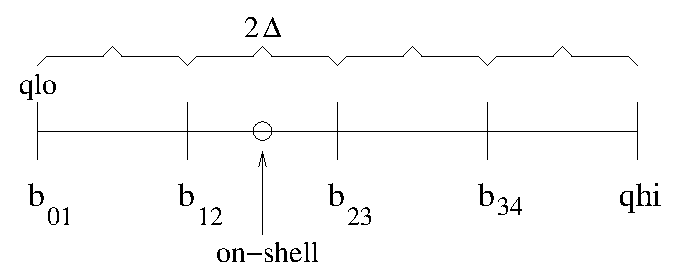
\includegraphics{redish.eps} \par}


\caption{\label{Fig:redish}Integration intervals for the evaluation of the
R-matrix}
\end{figure}

\end{itemize}

\subsubsection*{OUT namelist:}

Magnitudes to be printed out.

\begin{itemize}
\item \textbf{dels}: phase shifts.
\item \textbf{aeoff}: off-shell amplitudes in the Wolfestein parametrization.
\item \textbf{aeon}: on-shell amplitudes in the Wolfestein parametrization.
\\
\\
\begin{tabular}{|c|c|c|}
\hline 
\multicolumn{3}{|c|}{aeoff}\\
\hline
Value&
Writen amplitudes&
Unit\\
\hline
\hline 
0&
-&
-\\
\hline 
1&
Isoscalar&
22\\
&
Isovector&
23\\
\hline 
2&
T=0&
34\\
&
T=1&
33\\
\hline 
3&
pn&
32\\
\hline
\end{tabular}~~~~\begin{tabular}{|c|c|c|}
\hline 
\multicolumn{3}{|c|}{aeon}\\
\hline 
Value&
Writen amplitudes&
Unit\\
\hline
\hline 
0&
-&
-\\
\hline 
1&
Isoscalar&
220\\
&
Isovector&
230\\
\hline 
2&
T=0&
340\\
&
T=1&
330\\
\hline 
3&
pn&
320\\
\hline
\end{tabular} \\
\\
Al these files have the format: \\
\\
\begin{tabular}{ccccccccc}
q&
Q&
Re(\( \cal {A} \))&
Img(\( \cal {A} \))&
Re(\( \cal {B} \))&
Img(\( \cal {B} \))&
\ldots{}&
Re(\( \cal {F} \))&
Img(\( \cal {F} \))\\
\end{tabular} \textbf{}
\item \textbf{moff}: off-shell amplitudes in tensor representation. Using
the notation of \cite{Cres01}, the following six independent amplitudes
are written: \( M_{00}^{(00)} \), \( M_{11}^{(01)} \), \( M_{00}^{(11)} \)
\( M_{20}^{(11)} \), \( M_{21}^{(11)} \) and \( M_{22}^{(11)} \)
. The names of the output files are built as:\[
M^{ab}_{kq}\, \rightarrow \, \mathrm{mabkq}.\mathrm{off}\]
The possible values of the variable \emph{moff} are: \\
\\
\begin{tabular}{|c|cc|}
\hline 
\multicolumn{3}{|c|}{moff}\\
\hline
\hline 
Value&
\multicolumn{2}{c|}{Written amplitude}\\
\hline 
0&
\multicolumn{2}{c|}{No output}\\
\hline 
1&
Isoscalar &
Isovector\\
\hline 
2&
T=0 &
T=1\\
\hline 
3&
pp  &
pn\\
\hline
\end{tabular}\\
\\
For each of the components, real and imaginary parts are written in
consecutive columns.
\item \textbf{mon}: on-shell amplitudes in tensor representation. The filenames
are the same, but using the extension \emph{.on}
\end{itemize}

\subsubsection*{PW namelist:}

Partial waves. 

\begin{itemize}
\item \textbf{is}: total spin of the NN system (0,1), S. 
\item \textbf{ll}: total orbital angular momentum, L.
\item \textbf{jj}: total angular momentum, J.
\end{itemize}

\subsubsection*{AMP namelist: }

Extra variables necessary to build the momentum space grid.

\begin{itemize}
\item \textbf{ifkq}: definition of the momentum transfered \( q \) and
total momentum \( Q \).
\end{itemize}
{\centering \begin{tabular}{|c|cc|}
\hline 
ifkq=0&
\( \vec{q}=\frac{\mathcal{K}'-\mathcal{K}}{\sqrt{2}} \) &
\( \vec{Q}=\frac{\mathcal{K}'+\mathcal{K}}{\sqrt{2}} \)\\
\hline
ifkq=1&
\( \vec{q}=\mathcal{K}'-\mathcal{K} \)&
\( \vec{Q}=\frac{\mathcal{K}'+\mathcal{K}}{2} \)\\
\hline
\end{tabular}\par}

\begin{itemize}
\item \textbf{xkmax}=step in \( Q \).
\item \textbf{xqmax}=step in \( q \).
\item \textbf{dk}: step in \( Q \) (default 0.1). 
\item \textbf{dq}: step in \( q \) (default 0.1) .
\item \textbf{theta}: angle between \( \vec{q} \) and \( \vec{Q} \), in
degrees (default 90).
\item \textbf{nth}: number of angles to calculate on-shell values (default
46). 
\end{itemize}

\subsection{MSO.in}


\subsubsection*{MSO namelist: }

\begin{itemize}
\item \textbf{tlab}: relative kinetic energy projectile-target in laboratory
system.
\item \textbf{offshell}: T/F
\item \textbf{kmt}: KMT (kmt=T) or Watson (kmt=F) potential. The former
contains the multiplying factor at/(at-1), with at the target atomic
number.
\item \textbf{igwf}: If T, calculates wavefunction up to lstore.
\item \textbf{lstore}: max. partial wave for wf.
\item \textbf{nr}: if nr is not 0, a relativistic correction is performed. 
\item \textbf{ucnr, ucni}: central renormalization constants.
\item \textbf{usnr, usni}: s.o. renormalization constants.
\end{itemize}

\subsubsection*{COUL namelist:}

\begin{itemize}
\item \textbf{coulomb}: Coulomb correction\\
=0: no coulomb\\
=1: coulomb amplitude and phase change included~\\
=2: coulomb amplitude, but not phase change\\
=3: realistic (HO shape) charge distribuion\\
=3: uniform charge sphere distribution
\item \textbf{rcut} :cut-off radius for subtracted momentum space method
\cite{Crespo90}.
\item \textbf{alfa, beta, gama}: parameters for the realistic charge distribution
of the form:\begin{equation}
\rho (q)=\left\{ 1-\gamma ^{2}q^{2}-\alpha q^{4}\right\} e^{-\beta q^{2}}
\end{equation}

\end{itemize}

\subsubsection*{HIGHORDER namelist:}

Specifications for high order calculations (second order onward)

\begin{itemize}
\item \textbf{second}:\\
= 1 SSA\\
= 2 DSA(local)\\
= 3 DSA (non local) \\
= 4 DSA (full nonlocal)
\item \textbf{isflip}:
\item \textbf{ich}: 
\item \textbf{ion2}: 
\item \textbf{lamx}:
\item \textbf{lbmx}: 
\item \textbf{l1mx}:
\item \textbf{lfmx}:
\item \textbf{rmaxr}: maximum radius
\item \textbf{quin}: maximum radius for inner region
\item \textbf{mquadi}: number of inner quad points (multiple of 6)
\item \textbf{mquado}: number of outer quad points (multiple of 6)
\end{itemize}

\subsubsection*{PROJ namelist:}

Projectile properties. Presently, the program only supports structureless
projectiles. Thus, unlike the target, no clusters can be defined.

\begin{itemize}
\item \textbf{massp}: mass number (in a.m.u.)
\item \textbf{zp}: charge
\end{itemize}

\subsubsection*{TARG namelist:}

Target properties

\begin{itemize}
\item \textbf{masst}: mass number (in a.m.u.)
\item \textbf{zt}: charge
\item \textbf{at}: number of nucleons
\item \textbf{ncluster}: number of clusters
\end{itemize}

\subsubsection*{CLUSTER namelist:}

After the \textbf{targ} namelist, \emph{ncluster} namelists will be
read. Each one contains the information required to construct the
density for one the clusters. Notice that the different cluster do
not neccesary have to use the same model density.

\begin{itemize}
\item \textbf{type}, \textbf{shape}: specify the kind of density. External
densities (type=1, shape=5) are read from fortran unit 4. The first
line contains the number of points (\emph{nramax}) and the step (\emph{drx}),
in free format. Then, nramax density points will be read, assuming
that the first one corresponds to the origin. \\
\begin{tabular}{|cc|cl|}
\hline 
\multicolumn{2}{|c|}{type}&
\multicolumn{2}{c|}{shape}\\
\hline
\hline 
0&
Numerical potential&
0&
Woods-Saxon\\
&
&
1&
Gauss\\
&
&
2&
Yukawa\\
&
&
3&
Hulthen\\
&
&
4&
cosh\\
&
&
5&
External\\
\hline 
1&
Analytical potential&
0&
Harmonic-oscillator s.p.\\
&
&
1&
Three-parameter Fermi\\
&
&
2&
G3 distribution\\
\hline
\end{tabular}
\item \textbf{nzclus}: number of protons within this cluster.
\item \textbf{nnclus}: number of neutrons within this cluster.
\end{itemize}

\subsubsection*{BSPARM namelist:}

For type=0, shape=0-4 the bsparm namelist is then read.

\begin{itemize}
\item \textbf{cmass, vmass}: core and bound particle masses.
\item \textbf{zc, zv}: core and bound particle charges.
\item \textbf{nramax}: number of integration steps.
\item \textbf{drx}: radial step for numerical integration.
\item \textbf{dmat}:fine tuning of interior-exterior matching. Usually input
0. {*} If no state found try increase of dmat to of order 10.
\item \textbf{nshell}: number of shells.
\end{itemize}

\subsubsection*{BSHELL namelist:}

Parameters for this specific shell.

\begin{itemize}
\item \textbf{bengy}: binding energy.
\item \textbf{vdepth}, \textbf{wr0, wal}: potential depth, radius and diffuseness.
\item \textbf{wls}: spin-orbit strength.
\item \textbf{is2}=2{*}valence particle spin \( s \).
\item \textbf{lmoma}= orbital angular momentum \( \ell  \).
\item \textbf{j2a} : 2{*}j, where \( j=\ell +s \).
\item \textbf{nodd}=number of nodes.
\item \textbf{norba}=occupation number of this shell.
\end{itemize}

\subsubsection*{BS3PF namelist:}

If type=1, shape=5 density is defined, a \textbf{\&bs3pf/} namelist
is then read. In configuration space, it obeys to the form:\begin{equation}
\label{Eq:rho-fermi}
\rho (r)=\rho _{0}\frac{1+w(r/c)^{2}}{\exp [(r-c)/z]}
\end{equation}
where \( \rho _{0} \) is a normalization constant and \( w,\, c,\, z \)
are free parameters. 

\begin{itemize}
\item \textbf{w3p, z3p}, \textbf{c3p}: Fermi parameters for protons.
\item \textbf{w3n, z3n, c3n}: Fermi parameters for neutrons.
\item \textbf{nramax}: number of radial points to calculate the density.
\item \textbf{drx}: step size (fm).
\end{itemize}

\subsubsection*{HOPARM namelist:}

For type=1, shape=0 densities, harmonic oscillator parameters are
read. First, a \textbf{hoparm} namelist is introduced, which currently
only contains the number of shells that will be next read by means
of \textbf{hoshell} namelists.

\begin{itemize}
\item \textbf{hoparm}: number of harmonic-oscillator shells to be read.
\end{itemize}

\subsubsection*{HOSHELL namelist: }

Provides the HO parameters and occupations numbers for each shell.

\begin{itemize}
\item \textbf{aap, aan}: HO parameters for protons and neutrons, respectively.
\item \textbf{zorba, norba}: occupation number (protons and neutrons) for
this shell.
\end{itemize}

\subsection{MST.in}


\subsubsection*{MST namelist:}

\begin{itemize}
\item \textbf{qmax: }
\item \textbf{tlab}: projectile energy in laboratory frame.
\item \textbf{thmin, thmax, dth}: angular range and step for calculated
cross sections.
\end{itemize}

\subsubsection*{QUAD1 namelist:}

\begin{itemize}
\item \textbf{qmaxr}: 
\item \textbf{quin}: 
\item \textbf{mquadi}: 
\item \textbf{mquado:}
\end{itemize}

\subsubsection*{QUAD2 namelist:}

\begin{itemize}
\item \textbf{qmaxrd}:
\item \textbf{quind}: 
\item \textbf{mquadid:}
\item \textbf{mquadod}: 
\end{itemize}

\subsubsection*{QUAD3 namelist:}

\begin{itemize}
\item \textbf{rmaxr} : 
\item \textbf{rin} :
\item \textbf{mrquadi} : 
\item \textbf{mrquado} : 
\end{itemize}

\subsubsection*{PROJ namelist:}

\begin{itemize}
\item \textbf{massp}: projectile mass
\item \textbf{zp}: projectile charge
\end{itemize}

\subsubsection*{TARG namelist:}

\begin{itemize}
\item \textbf{masst}: target mass
\item \textbf{zt}: target charge 
\item \textbf{ncl}: number of clusters.
\item \textbf{inelcb}: ?????
\item \textbf{nustates}: total number of states.
\item \textbf{quais(1:nustates-1)}: vector array to select those \( J^{\pi } \)
(inelastic) components of the wavefunction that will be taken into
account in the calculations. \( quais(i)\neq 0 \) means that component
\( i \) will be included.
\item \textbf{irho}: ???
\end{itemize}

\subsubsection*{KAPAS namelist:}

\begin{itemize}
\item \textbf{k0000, k1100, k0111, k1120, k1121, k1122}: If \emph{kabkq}=1
the tensor component \( t^{(ab)}_{\kappa q}(\omega \, \vec{\Delta }) \)
of the NN amplitude will be taken into account.
\end{itemize}

\subsubsection*{TCLUS namelist: }

\begin{itemize}
\item \textbf{mtclus}: mass of this cluster (u.m.a.)
\item \textbf{spin}: cluster intrinsic spin
\item \textbf{ztclus}: cluster charge
\end{itemize}

\section{Test case and set up}

The namelist input style provides a very intuitive description of
the input file by itself. 


\subsection*{Example of input file}

\verbatiminput{nnamp.dat}

\&system tcm=67.5 nnpot='paris' /

The first namelist (\textbf{\&system/}) sets the center of mass energy
of the colliding nucleons and the kind of NN potential. In this example
the variable \textbf{jmax} is not specified and so it is understood
that partial waves are to be given explicitly in this input file.
\\


\&out dels=1 aeon=0 aeoff=0 mon=2 moff=2 /

The namelist \textbf{out} specifies the information that is going
to be calculated and printed out by the program. In this example the
phase shifts (\textbf{dels=1}) and the T=0 and T=1 components of the
on- and off-shell NN amplitude in tensor representation.\\


\&kmat hw=0.5 b01=0. b34=30. ,n1=5 n2=6 n3=15 n4=6, s=1.0, qlo=0.,
qhi=1000. /

Then, namelist \textbf{\&kmat/} it is provided the parameters required
to calculate the R-matrix. In particular, the boundaries of the regions
defined in the integration (\textbf{b01}, \textbf{b34} and \textbf{hw})
as shown in Fig.\ \ref{Fig:redish}. Also the number of quadrature
points is given (n1,n2,n3,n4). \\


\&pw is=0 ll=0 jj=0 /

\&pw is=1 ll=1 jj=0 /

\&pw is=0 ll=1 jj=1 /

\&pw is=1 ll=1 jj=1 /

\&pw is=1 ll=0 jj=1 /

\&pw is=0 ll=2 jj=2 /

\&pw is=1 ll=2 jj=2 /

\&pw is=1 ll=1 jj=2 /

\&pw is=0 ll=3 jj=3 /

\&pw is=1 ll=3 jj=3 /

\&pw is=1 ll=2 jj=3 /

\&pw is=0 ll=4 jj=4 /

\&pw is=1 ll=4 jj=4 /

\&pw is=1 ll=3 jj=4 /

\&pw is=0 ll=5 jj=5 /

\&pw is=1 ll=5 jj=5 /

\&pw is=1 ll=4 jj=5 /

\&pw is=0 ll=6 jj=6 /

\&pw is=1 ll=6 jj=6 /

\&pw is=-1 ll=0 jj=0 / 

Then a set of namelist \&pw/ are read in order to provide the partial
waves considered.

~

\&amp ifkq=1 xkmax=2.0 xqmax=3.5 dk=0.2 dq=0.2 theta=45. nth=90, 

itype=2 icase=2 /

Finally, the \textbf{\&amp/} namelist gives the required parameters
for the evaluation of the T-matrix starting from the R-matrix.


\newpage
\subsection*{Example of output file dels.dat}

\verbatiminput{dels.dat}

\bibliographystyle{unsrt}
\bibliography{referRC}

\end{document}
